\documentclass[11pt]{article}
\usepackage[margin=1in]{geometry}
\usepackage{amsmath,amssymb}
\usepackage{graphicx}
\usepackage{booktabs}
\usepackage{hyperref}

% Shared macros loaded by main.tex via % Shared macros loaded by main.tex via % Shared macros loaded by main.tex via \input{macros}
\newcommand{\R}{\mathbb{R}}
\newcommand{\norm}[1]{\left\lVert #1 \right\rVert}

\newcommand{\R}{\mathbb{R}}
\newcommand{\norm}[1]{\left\lVert #1 \right\rVert}

\newcommand{\R}{\mathbb{R}}
\newcommand{\norm}[1]{\left\lVert #1 \right\rVert}


\title{A Mini \LaTeX{} Tutorial}
\author{Learn by editing this project}
\date{\today}

\begin{document}
\maketitle

\begin{abstract}
This starter project is a short hands-on tutorial.
Each section shows a common pattern---multi-file input, macros, figures,
tables, cross-references, math, and BibTeX---and briefly explains how the
source produces what you see in the PDF. Edit any file in the tree, compile,
and compare the output with the notes below.
\end{abstract}

\tableofcontents
\newpage

\section{Split the source into files}
\label{sec:intro}

This section lives in \texttt{sections/introduction.tex}.
\texttt{main.tex} pulls it in with:

\begin{verbatim}
\section{Split the source into files}
\label{sec:intro}

This section lives in \texttt{sections/introduction.tex}.
\texttt{main.tex} pulls it in with:

\begin{verbatim}
\section{Split the source into files}
\label{sec:intro}

This section lives in \texttt{sections/introduction.tex}.
\texttt{main.tex} pulls it in with:

\begin{verbatim}
\input{sections/introduction}
\end{verbatim}

That is the usual way to keep a growing paper readable: one file per section,
plus a short root file that only sets up packages and the document skeleton.

\subsection{Shared macros}
Commands such as \texttt{\textbackslash R} and \texttt{\textbackslash norm}
are defined once in \texttt{macros.tex} (loaded near the top of
\texttt{main.tex}). After that, you can write $\R$ or $\norm{x}$ anywhere
without repeating the definition.

\subsection{A labeled equation}
For $x \in \R$, a classic identity is
\begin{equation}
\label{eq:euler}
  e^{i\pi} + 1 = 0.
\end{equation}
The \texttt{\textbackslash label\{eq:euler\}} makes it possible to point back
here later with \texttt{\textbackslash eqref\{eq:euler\}} or
\texttt{\textbackslash ref\{eq:euler\}}. Cross-references update after you
compile again (a second pass is normal).

\subsection{Citations from a \texttt{.bib} file}
A citation like \cite{lamport94} comes from \texttt{references.bib}.
After the first successful compile, run your bibliography tool (BibTeX), then
compile again so the reference list and in-text citations resolve.

\end{verbatim}

That is the usual way to keep a growing paper readable: one file per section,
plus a short root file that only sets up packages and the document skeleton.

\subsection{Shared macros}
Commands such as \texttt{\textbackslash R} and \texttt{\textbackslash norm}
are defined once in \texttt{macros.tex} (loaded near the top of
\texttt{main.tex}). After that, you can write $\R$ or $\norm{x}$ anywhere
without repeating the definition.

\subsection{A labeled equation}
For $x \in \R$, a classic identity is
\begin{equation}
\label{eq:euler}
  e^{i\pi} + 1 = 0.
\end{equation}
The \texttt{\textbackslash label\{eq:euler\}} makes it possible to point back
here later with \texttt{\textbackslash eqref\{eq:euler\}} or
\texttt{\textbackslash ref\{eq:euler\}}. Cross-references update after you
compile again (a second pass is normal).

\subsection{Citations from a \texttt{.bib} file}
A citation like \cite{lamport94} comes from \texttt{references.bib}.
After the first successful compile, run your bibliography tool (BibTeX), then
compile again so the reference list and in-text citations resolve.

\end{verbatim}

That is the usual way to keep a growing paper readable: one file per section,
plus a short root file that only sets up packages and the document skeleton.

\subsection{Shared macros}
Commands such as \texttt{\textbackslash R} and \texttt{\textbackslash norm}
are defined once in \texttt{macros.tex} (loaded near the top of
\texttt{main.tex}). After that, you can write $\R$ or $\norm{x}$ anywhere
without repeating the definition.

\subsection{A labeled equation}
For $x \in \R$, a classic identity is
\begin{equation}
\label{eq:euler}
  e^{i\pi} + 1 = 0.
\end{equation}
The \texttt{\textbackslash label\{eq:euler\}} makes it possible to point back
here later with \texttt{\textbackslash eqref\{eq:euler\}} or
\texttt{\textbackslash ref\{eq:euler\}}. Cross-references update after you
compile again (a second pass is normal).

\subsection{Citations from a \texttt{.bib} file}
A citation like \cite{lamport94} comes from \texttt{references.bib}.
After the first successful compile, run your bibliography tool (BibTeX), then
compile again so the reference list and in-text citations resolve.

\section{Figures, tables, and display math}
\label{sec:results}

\subsection{Figures}
Figure~\ref{fig:diagram} is the PNG at \texttt{figures/diagram.png}, included
with the \texttt{graphicx} package:

\begin{verbatim}
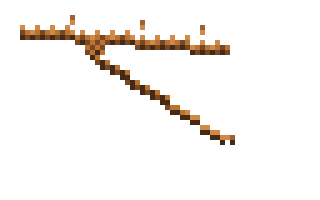
\includegraphics[width=0.62\textwidth]{figures/diagram.png}
\end{verbatim}

\begin{figure}[ht]
  \centering
  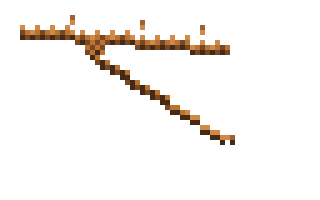
\includegraphics[width=0.62\textwidth]{figures/diagram.png}
  \caption{A small pixel figure shipped with this starter project.}
  \label{fig:diagram}
\end{figure}

Put assets under \texttt{figures/} (or any folder you prefer) and keep the path
in \texttt{\textbackslash includegraphics} in sync with the tree.

\subsection{Tables}
Tables are ordinary \texttt{tabular} environments. The rules below come from
\texttt{booktabs} (\texttt{\textbackslash toprule}, \texttt{\textbackslash midrule},
\texttt{\textbackslash bottomrule}):

\begin{table}[ht]
  \centering
  \begin{tabular}{lrr}
    \toprule
    Method & Error & Time (s) \\
    \midrule
    Baseline & 0.041 & 1.2 \\
    Improved & 0.018 & 1.5 \\
    \bottomrule
  \end{tabular}
  \caption{A compact comparison table using \texttt{booktabs}.}
  \label{tab:compare}
\end{table}

Refer to the table with \texttt{\textbackslash ref\{tab:compare\}} $\to$
Table~\ref{tab:compare}.

\subsection{Aligned math}
Multi-line displays use \texttt{align} from \texttt{amsmath}. The
\verb|&| character marks the alignment point and \verb|\\|
breaks the line:

\begin{align}
  \norm{Ax - b}_2^2
    &= (Ax - b)^\top (Ax - b) \\
    &= x^\top A^\top A x - 2 b^\top A x + b^\top b.
\end{align}

\subsection{Lists and footnotes}
\begin{itemize}
  \item Upload a folder to mirror a local project layout.
  \item Drag files between folders in the file tree.
  \item Keep experimenting: change numbers in Table~\ref{tab:compare} and
        recompile to see the PDF update.
\end{itemize}

A short footnote can hold an aside.\footnote{Footnotes are written with
\texttt{\textbackslash footnote\{...\}} right where the mark should appear.}
Equation~\eqref{eq:euler} was introduced in Section~\ref{sec:intro}.

\section{Where to go next}
\label{sec:next}

\subsection{A heavier starter: DummyHippo}
When this tutorial feels too small, try \textbf{DummyHippo}: a deliberately
heavy multi-file project (nested chapters, TikZ/PGFPlots, denser math, and a
larger bibliography). Use it as a tougher starting point once you are
comfortable with the patterns above.

Download or clone the folder from:
\begin{center}
\url{https://github.com/martino-vic/undertwig/tree/main/DummyHippo}
\end{center}

To bring it into this workspace:
\begin{enumerate}
  \item Open that link and download the \texttt{DummyHippo} folder
        (clone the repository, or use GitHub's download / raw folder copy).
  \item In the app, click \textbf{Import new project}.
  \item Choose the local \texttt{DummyHippo} directory---the one that contains
        \texttt{main.tex} (not only an inner \texttt{chapters} folder).
  \item Compile with \textbf{Convert}. For citations, run
        \textbf{Update Bibliography}, then \textbf{Convert} again.
\end{enumerate}

\subsection{Bibliography wrap-up}
Classic references such as \cite{lamport94} and \cite{knuth84} are resolved from
\texttt{references.bib} via
\begin{verbatim}
\bibliographystyle{plain}
\bibliography{references}
\end{verbatim}
at the end of \texttt{main.tex}. Remember the usual loop: compile $\to$
bibliography tool $\to$ compile again.

\subsection{Thanks}
Thanks for reading through all of this---now open a blank section and start
writing your own material, or import DummyHippo if you want a tougher compile.


\bibliographystyle{plain}
\phantomsection
\addcontentsline{toc}{section}{\refname}
\bibliography{references}

\end{document}
